\documentclass[a4paper,10pt]{article}

%\usepackage{xltxtra}
\usepackage{fontspec, unicode-math}
\usepackage{amsmath}
\usepackage{hyperref}

\usepackage[]{biblatex}
\addbibresource{Notes-ref.bib}

\usepackage{tikz}
\usetikzlibrary{patterns,decorations.pathmorphing,shapes,arrows,positioning,decorations.pathreplacing,calc,backgrounds,external,spy}

\setromanfont[Mapping=tex-text]{Linux Libertine O}
% \setsansfont[Mapping=tex-text]{DejaVu Sans}
% \setmonofont[Mapping=tex-text]{DejaVu Sans Mono}

\title{Vacuum Electronics in Cylindrical Coordinates}
\author{Kristinn Torfason}
\date{\today}

\newcommand{\ud}{\mathrm{d}}

\begin{document}
\maketitle
\newpage

\section{Electric Field}
The Laplace equation in cylindrical coordinates is
\begin{equation}
 \nabla^2\Phi = \frac{1}{r}\frac{\delta}{\delta r}\left( r \frac{\delta\Phi}{\delta r}\right)
              + \frac{1}{r^2}\frac{\delta^2\Phi}{\delta \theta^2} + \frac{\delta^2\Phi}{\delta z} = 0\, .
\end{equation}
Due to symmetry in \(\theta\) and \(z\) we have
\begin{equation}
 \Phi = \Phi(r)\, ,
\end{equation}
or
\begin{equation}
 \nabla^2\Phi(r) = \frac{1}{r}\frac{\delta}{\delta r}\left( r \frac{\delta\Phi(r)}{\delta r}\right) = 0\, .
\end{equation}
Integration yields,
\begin{equation}
  \frac{\delta \Phi(r)}{\delta r} = \frac{A}{r}\, ,
\end{equation}
where \(A\) is a constant. A second integration then gives,
\begin{equation}
  \Phi(r) = A\ln(r) + B\, ,
\end{equation}
where \(B\) is also a constant.
\begin{figure}[!h]
  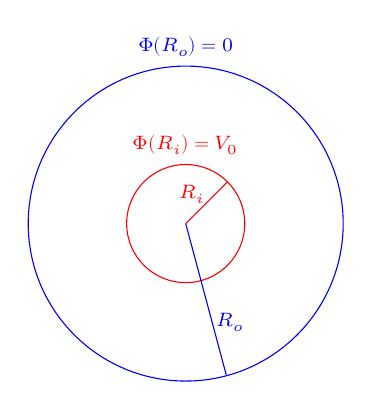
\begin{tikzpicture}
    \draw[red] (0, 0) circle (0.75cm);
    \draw[blue] (0, 0) circle (2.0cm);
    
    \draw[red] (0, 0) -- (45:0.75cm) node[midway, left, font=\scriptsize, xshift=3pt, yshift=3pt] {\(R_i\)};
    \draw[blue] (0, 0) -- (-75:0.75cm);
    \draw[blue] (-75:0.75cm) -- (-75:2.0cm) node[midway, right, font=\scriptsize, xshift=-2.5pt, yshift=2pt] {\(R_o\)};
    
    \node[font=\scriptsize, above, red] at (90:0.75cm) {\(\Phi(R_i) = V_0\)};
    \node[font=\scriptsize, above, blue] at (90:2.00cm) {\(\Phi(R_o) = 0\)};
  \end{tikzpicture}
  \centering
  \caption{A schematic illustration of the system.}
  \label{fig:system}
\end{figure}
The boundary conditions seen in Fig.~\ref{fig:system} are \(\Phi(R_i) = V_0\) and \(\Phi(R_o) = 0\). Using them to solve for the constants gives
\begin{equation}
  B = V_0\frac{\ln(R_o)}{\ln(R_o/R_i)}\, ,
\end{equation}
and
\begin{equation}
  A = \frac{V_0}{\ln(R_i/R_o)}\, .
\end{equation}
The electric field is then
\begin{equation}
 \vec{E} = - \vec{\nabla}\Phi
 = -\left(\frac{\delta \Phi}{\delta r}\hat{r} + \frac{1}{r}\frac{\delta\Phi}{\delta \theta}\hat{\theta} + \frac{\delta\Phi}{\delta z}\hat{z} \right)\, ,
\end{equation}
or
\begin{equation}
 \vec{E} = \frac{V_0}{\ln(R_o/R_i)}\frac{\hat{r}}{r}
         = \frac{V_0}{\ln(R_o/R_i)} \frac{\cos(\theta)\hat{x} + \sin(\theta)\hat{y}}{r}\, .
\end{equation}

\section{Emission}
The emission process checks the angle between the positon vector (black solid line) and the acceleration (\textcolor{violet}{violet} dashed line) (see Fig.~\ref{fig:angle}). If the angle \(\theta\) is greater than \(\pi/2\) then emission can occur.
\begin{figure}[!h]
  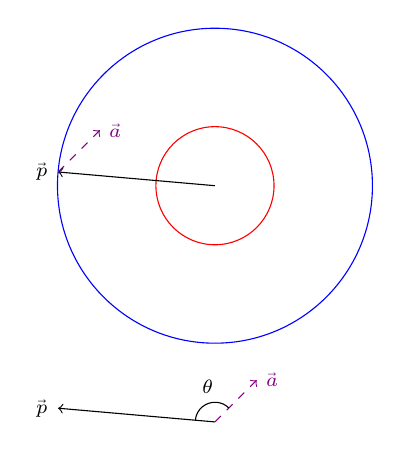
\begin{tikzpicture}
    \draw[red] (0, 0) circle (0.75cm);
    \draw[blue] (0, 0) circle (2.0cm);
    
    \draw[black, ->] (0:0) -- (175:2.0cm) node[left, font=\scriptsize] {\(\vec{p}\)};
    \draw[violet, dashed, ->] (175:2.0cm) -- ++(45:0.75cm) node[right, font=\scriptsize] {\(\vec{a}\)};
    
    \begin{scope}[yshift=-3cm]
     \draw[black, ->] (0:0) -- (175:2.0cm) node[left, font=\scriptsize] {\(\vec{p}\)};
     \draw[violet, dashed, ->] (0:0cm) -- ++(45:0.75cm) node[right, font=\scriptsize] {\(\vec{a}\)};
     \draw (175:0.25cm) arc (175:45:0.25cm) node[above, midway, font=\scriptsize] {\(\theta\)};
    \end{scope}
  \end{tikzpicture}
  \centering
  \caption{Angle between position and acceleration.}
  \label{fig:angle}
\end{figure}
\end{document}